\chapter{Integration of Transfer Learning}\label{In}
In this chapter, two versions of the \ac{PCTKVM} are proposed.
The \acs{PCTKVM} which handles the $\theta$ as a fixed parameter and the \acs{PCTKVM}\textsubscript{$\theta$Est}, which does a theta estimation.
The extensions 'TK' to original term \acs{PCVM} should indicate the new kernel approach to address the transfer learning problem.
As already mentioned in chapter \ref{Tl} there are various solutions to solve the transfer learning problem.
Revisiting section \ref{TlSecHomo}, the homogeneous transfer learning problem can be summarized in four approaches: Instance-Transfer, Symmetric-Feature-Transfer, Asymmetric-Feature-Transfer, and Relational-Knowledge-Transfer.\newline
However, Long et al. proposed in \cite{Long.2015}, transfer kernel learning as another approach-category.
Nevertheless, that the relational knowledge approach, transfers information through relationships between the source and target data, the \acs{TKL} approach suits well in this category.
Furthermore, because it needs target data for the learning process and according to the definition of transductive transfer learning, it can be categorized as transductive transfer setting.\\
The main idea of it is to approximate the kernel of the training set with the kernel of the test set via the Nyström kernel approximation.\cite{Long.2015}
On the other hand \cite{Schleif.2015}, proposed a \acs{PCVM} with linear costs which is also achieved via the Nyström approximation.
Therefore, it seems reasonable, to integrate another interpretation of the Nyström approximation into the \acs{PCVM}.\\
Another advantage is that \acs{TKL} is very simple when it comes to dataset usage.
According to \ref{TlSecDef} there are transfer learning solutions which need pre-labeled test data.
As we will see in the following, the \acs{TKL} using only the training and an unlabeled test dataset to compute the transfer kernel and therefore has an 'easy' handling.\newline
However, before going into the approach itself, the underlying technique should be discussed.
See section \ref{EmSubSecKernel} for details to kernels and the Gram matrix.
\section{Nyström Approximation}\label{InSecNysMeth}
The main Problem by computing eigenvalues and eigenvectors is that optimal eigenvalue decomposition has a time complexity of $\mathcal{O}(N^3)$ and alternative approaches must be found.
The Nyström Method was originally made for solving the eigenvalue equation, which can be seen in equation \eqref{EqEigsEq}.\cite{Zhang.2008}\\
It is done by randomly selecting $N$ observations (rows/columns) without replacement out of $\mathbf{K}$ for calculating the approximation.\cite{Williams.2000}
Considering a symmetric positive semi definite kernel $k(\mathbf{z},\mathbf{x})$ which satisfies Mercers Theorem, then $\mathbf{K}$ can be represented as:\cite{Williams.2000}
\begin{equation}\label{EqKernelRep}
	k(\mathbf{z},\mathbf{x}) = \sum_{i=1}^{D}\lambda_i\phi_i(\mathbf{z})\phi_i(\mathbf{x}) 
\end{equation}
With $D < \infty$ as the number of feature space dimensions and $\lambda_1 \ge \lambda_2\ge\dots\ge0$ as the sorted eigenvalues and $\phi_i$ as eigenfunctions.
As consequence of Mercer follows that  $\lambda_i$ and $\phi_i$ have to satisfy the eigenvalue equations:
 \begin{equation}\label{EqEigsEq}
	\int_{i=1}^{D} k(\mathbf{x},\mathbf{z})\phi_i(\mathbf{z})p(\mathbf{z})d\mathbf{x} = \lambda_i\phi_i(\mathbf{x})
\end{equation}
With $p(\mathbf{z})$ as the probability density of the input vector $\mathbf{z}$.
Furthermore, the orthogonality conditions are satisfied with:\cite[p. 59]{Scholkopf.2001}
\begin{equation}\label{EqEigsOrt}
	\int \phi_i(\mathbf{z})\phi_j(\mathbf{z})p(\mathbf{z})d\mathbf{z} = \delta
\end{equation}
If a kernel as defined above is given, then an empirical estimate can be done by, drawing an identical and independently sample ${\mathbf{z}_1,\dots,\mathbf{z}_N}$ from $p(\mathbf{z})$.
The integral can be rewritten as an empirical estimate:\cite{Williams.2000}
\begin{equation}\label{EqEigsEmp}
	\sum_{k=1}^{N}\frac{k(\mathbf{x},\mathbf{z}_k)\phi_i(\mathbf{z}_k)}{N} \approx \lambda_i\phi_i(\mathbf{x})
\end{equation}
Where $N$ is the number of sampled observation from the kernel and the $N$ orthogonal eigenfunctions.
If we consider the N columns from $\mathbf{K} \in \mathbb{R}^{K\times K}$ as separate kernel matrix $\mathbf{K}^{(N)}$ with size $N\times N$ and elements $K_{ij}^{(N)}=K(\mathbf{z_i,z_j})$ for $i,j=\{1,\dots,N\}$, then we can use this for the eigenvalue problem of the sample kernel:\cite{Williams.2000}
\begin{equation}\label{EqEigsProb}
	\mathbf{K}^{(N)}\mathbf{U}^{(N)} = \mathbf{U}^{(N)}\mathbf{\Lambda}^{(N)}
\end{equation} 
With $\mathbf{U}^{(N)} \in \mathbb{R}^{N\times N}$ as eigenvectors and $\boldsymbol{\Lambda}^{(N)}$ as a diagonal matrix with the eigenvalues for the small kernel with $\lambda_1^{(N)}\ge\lambda_2^{(N)}\ge\dots\lambda_N^{(N)} \ge0$.
If we consider points within the kernel $K^{(N)}$, then $\mathbf{x}$ can be replaced with $\mathbf{z}_j$.
Continuing with matching \eqref{EqEigsEmp} against \eqref{EqEigsProb} then the following approximation can be obtained:\cite{Williams.2000}
\begin{equation}\label{EqEigsFuncAprox}
	\phi_i(\mathbf{z}_j) \approx \sqrt{N}U_{ij}^{(N)}
\end{equation}
Finally, by using $\phi_i(x_k)$ in \eqref{EqEigsEmp} the approximation for any eigenvector or eigenvalue can be given by:
\begin{equation}\label{EqEigsValAprox}
	\phi_i(\mathbf{x})\approx\frac{\sqrt{N}}{\lambda_i^{(N)}}\sum_{k=1}^{N}k(\mathbf{x},\mathbf{z_k})U_{k,i}^{(N)}, \>\>\>\>\> \lambda_i \approx \frac{\lambda_i^{(N)}}{N}
\end{equation}
With this, the $i$-th eigenfunctions and eigenvalues can be approximated by calculating the sample kernel.\cite{Williams.2000}
As a consequence, the eigenfunctions and eigenvalues of the whole kernel can be approximated.
\subsection{Nyström Kernel Learning}\label{InSubSecNyKerneLearning}
Willams and Seeger extended the work of Nyström to speed up kernel machines.
The problem with kernel-based predictors, e.\,g., \acs{SVM}, is similar to the eigenvalue decomposition problem from section \ref{InSecNysMeth}
It requires the computational complexity of $\mathcal{O}(N^3$) in the worst case, to find a solution.\cite{Williams.2000}\\
With the Nyström approximation, the complexity for predictors can be bound by $\mathcal{O}(M^3N)$ with using a smaller system with size $M$, where $M<N$.\cite{Williams.2000}\\	
Now the goal is to create a low-rank approximation Matrix $\tilde{\mathbf{K}}$ of the original $N\times N$ kernel matrix $\mathbf{K}$.
Revisiting section \ref{InSecNysMeth}, by using the technique of Nyström, a kernel $\mathbf{K}$ which satisfies Mercer's theorem is needed.\cite{Williams.2000}
Furthermore, we draw $M$ \acs{IID} samples of $\mathbf{K}$ and therefore we can rewrite the symmetric kernel according to:\cite{Nemtsov.2016}
\begin{equation}\label{EqNystKernelParts}
	\mathbf{K} = 
	\begin{bmatrix}
		 \mathbf{K}_{M,M}\>\>\>\> \mathbf{K}_{M,N-M} \\
		 \mathbf{K}_{N-M,M}\>\>\>\> \mathbf{K}_{N-M,N-M}
	\end{bmatrix}
\end{equation}
Where $\mathbf{K}_{M,M}$ is the sample matrix and $\mathbf{K}_{N-M,M}$ is the crossdata-matrix of $\mathbf{K}$ and the rest of the data $\mathbf{K}_{N-M,N-M}$.
Because $\mathbf{K}$ is symmetric $\mathbf{K}_{N-M,M} = (\mathbf{K}_{M,N-M})^T$.
Furthermore, $\mathbf{K}_{N-M,N-M}$ is the part of the kernel which is not sampled or 'used' for the approximation, as we will see.\\
Motivated by the general eigenvalue problem, which can be obtained from \cite[p. 221]{Hartmann.2015} and shown in \eqref{EqEigsProb}, a kernel can be approximated through another kernel $\tilde{\mathbf{K}} = \tilde{\mathbf{U}}\tilde{\mathbf{\Lambda}}\tilde{\mathbf{U}}^T=\sum_{i=1}^{p}\tilde{\lambda}_i^{(N)}\tilde{\mathbf{u}}_i^{(N)}(\tilde{\mathbf{u}}_i^{(N)})^T$.\cite{Williams.2000}
With the approximated eigenvalues and eigenvectors as $\tilde{\lambda}_i^{(N)}$ and $\tilde{\mathbf{u}}_i^{(N)}$ respectively.\\
Therefore, we proceed with the equations to approximate the eigenvalues and eigenvectors.
By applying the equations of \eqref{EqEigsFuncAprox} and \eqref{EqEigsValAprox}, the approximation is based on the eigenvalues and eigenvectors of the sample matrix and can be made with:\cite{Zhang.2008}
\begin{equation}\label{EqNystEigsApprox}
	\begin{gathered}
			\tilde{\lambda}_i^{(N)} = \frac{N}{M}\lambda_i^{(M)} \>\>\>\>\> \sim \>\>\>\>\> \boldsymbol{\Lambda}^{(N)} =\frac{N}{M}\boldsymbol{\Lambda}^{(M)}\\
			\tilde{\mathbf{u}}_i^{(N)} = \sqrt{\frac{M}{N}}\frac{1}{\lambda_i^{(M)}}\mathbf{K}_{N,M}\mathbf{u}_i^{(M)}\>\>\>\>\> \sim \>\>\>\>\> \mathbf{U}^{(N)} = \sqrt{\frac{M}{N}}\mathbf{K}_{N,M}\mathbf{U}^{(M)}(\boldsymbol{\Lambda}^{(N)})^{-1}
	\end{gathered}
\end{equation}
With $i=1,\dots,N$ and $u_i^{(M)}$ and $\lambda_i^{(M)}$ from the eigenproblem (Eq. \eqref{EqEigsProb}).
After obtaining the approximated eigenvalues and vectors, the full approximated kernel can be restored:\cite{Williams.2000}\cite{Zhang.2008}
\begin{equation}\label{EqNystKernelEigsApprox}
	\tilde{\mathbf{K}} = \bigg(\sqrt{\frac{M}{N}}\mathbf{K}_{N,M}\mathbf{U}^{(M)}(\boldsymbol{\Lambda}^{(N)})^{-1}\bigg)\bigg(\frac{N}{M}\boldsymbol{\Lambda}^{(M)}\bigg)\bigg(\sqrt{\frac{M}{N}}\mathbf{K}_{N,M}\mathbf{U}^{(M)}(\boldsymbol{\Lambda}^{(N)})^{-1}\bigg)^T 
\end{equation}
With the use of $\tilde{\mathbf{K}} = \tilde{\mathbf{U}}\tilde{\mathbf{\Lambda}}\tilde{\mathbf{U}}^T$ in equation \eqref{EqNystEigsApprox} the approximation can be rewritten as:
\begin{equation}\label{EqNystKernelApprox}
		\tilde{\mathbf{K}} = \mathbf{K}_{N,M}(\mathbf{K}_{M,M})^{-1}\mathbf{K}_{M,N}
\end{equation}
From \eqref{EqNystKernelApprox} one can see that the kernel approximation can fully be made by the sample matrix and the submatrix $K_{N-M, N}$ of the 'original' kernel.\cite{Williams.2000}\\
The error bound of the Nyström Kernel approximation is $E_{Nys}=||\mathbf{K}-\tilde{\mathbf{K}}||$.\cite{He.2017}
This error can be minimized by choosing the samples carefully and a reasonable amount of it.
If the original Kernel $\mathbf{K}$ has rank $M$ and the samples are linearly independent columns from the kernel, then the approximation is exact.
As a consequence, from above choosing only $P$ samples with $P< M$ the error rises the fewer columns are chosen.\cite{Williams.2000}\\
The problem with choosing (sampling) columns/rows is that we usually do not know which columns are linearly independent.
Therefore, some sampling methods or approximations were made in the past to make this sampling more deterministic.
For example \cite{Kumar.2012}, which tries to find good samples through various sampling techniques, or \cite{Li.2015}, where the authors are drawing a large sample but approximate the submatrices with \ac{SVD}.\\
To summarize the Nyström Kernel approximation, first, we select $P$ of $N$ 'good' samples from the data and reorganizing the kernel according to \eqref{EqNystKernelParts}.
At this point, we have two options:
First calculating the kernel just for $\mathbf{K}_{M, M}$ and the submatrix ${K}_{N-M, M}$, continuing with approximate the eigenvectors and eigenvalues and finally calculating the approximated kernel $\tilde{\mathbf{K}}$ \eqref{EqNystKernelEigsApprox}.
Second calculate the approximation directly from the kernel as shown in equation \eqref{EqNystKernelApprox}. Note that the second approach needs a matrix inversion of the kernel, which should be considered for the use with large datasets.
\section{Domain Invariant Kernel Learning}\label{InSecTrans}
The \ac{TKL} approach is made by Long et al. in  \cite{Long.2015}\footnote{\url{http://ise.thss.tsinghua.edu.cn/~mlong/doc/transfer-kernel-learning-tkde15.zip}}.
They are interpreting the kernel approximation from a different point of view.
The main idea is to see the train dataset-matrix, which has to be approximated by the test dataset. Proceed by finding eigenvalues in a way that the difference between the approximation and ground truth training kernel will be minimal, which results in aligned marginal probability distributions.
This forms a domain invariant kernel for transfer learning.\cite{Long.2015}
The principal process is shown in figure \ref{FigTKLApp}.\newline 
From the above consider $\mathbf{z}$ as $\mathbf{Z}=\{\mathbf{z}_1,\dots,\mathbf{z}_{N}\}$ as training dataset which is sampled from $p(\mathbf{Z})$ within training domain $\mathcal{Z}$ and $\mathbf{x}$ as $\mathbf{X}=\{\mathbf{x}_1,\dots,\mathbf{x}_{M}\}$ as test dataset sampled from $p(\mathbf{X})$ within the test domain $\mathcal{X}$.
The definitions are based on \ref{TlSecDef}.
The associated kernels are $\mathbf{K}_\mathcal{Z}$ for training and $\mathbf{K}_\mathcal{X}$ for testing.\\
A fundamental insight of the \acs{RKHS} is that any \ac{PSD} kernel can be reconstructed based on the eigensystem of it. Furthermore, any new datasets can be incorporated into a kernel.\cite{Long.2015}\\
This means given a kernel $\mathbf{K}_\mathcal{X}$ of the dataset, using only the eigensystem $\{\lambda_i,\phi_i(\mathbf{x})\}$ the kernel can be evaluated by any new data point $\mathbf{z}$ and finally generating the kernel $\mathbf{K}_\mathcal{Z}$.
Again we could approximate the needed training kernel through:\cite{Long.2015}
\begin{equation}\label{EqTrainTestApprox}
	\mathbf{K}_\mathcal{Z} \simeq \mathbf{U}_\mathcal{Z}\boldsymbol{\Lambda}_\mathcal{X} \mathbf{U}_\mathcal{Z}^T = \mathbf{K}_\mathcal{ZX}\mathbf{K}_\mathcal{X}^{-1}\mathbf{K}_\mathcal{XZ}
\end{equation}
Where $\mathbf{U}_\mathcal{Z}$ as eigenvectors of the training kernel, $\boldsymbol{\Lambda}_\mathcal{X}$ as eigenvalues of the target kernel and $\mathbf{K}_\mathcal{ZX} = \mathbf{K}_\mathcal{ZX}^T$.
This is, in fact, a rewritten version of \eqref{EqNystKernelApprox}.\\
However, there might be a major problem.
Regarding two feature spaces, especially when it comes to transfer learning, then we have made the assumption that test and training feature spaces following different probability distributions.
This means that $P(\mathbf{Z})\neq P(\mathbf{X})$ and as a consequence the error of the approximation from \eqref{EqTrainTestApprox} can be arbitrarily large.\cite{Long.2015}\\
However, to align the distribution difference is one goal of transfer learning.
The main improvement which is done by Long et al. is to tackle this problem and to learn the domain invariant approximated kernel $\mathbf{\expP{K}}_{\mathcal{A}}$.\cite{Long.2015}
\begin{figure}
	\centering
	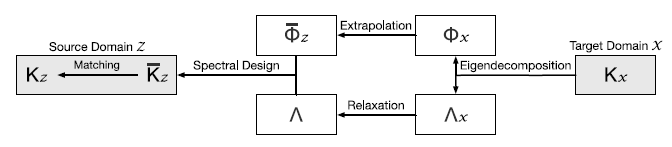
\includegraphics[width=.8\linewidth]{figures/ProcessTKL.png}
	\caption[Tranfer Kernel Learning Process]{The process of the Domain Invariant Kernel learning. It illustrates the relaxation of eigenvalues and extrapolation of eigenvectors. The tasks relaxation and extrapolation are forming the new domain invariant kernel.\cite{Long.2015}}
	\label{FigTKLApp}
\end{figure}
\subsection{Learning Approach}\label{InSubSecLearnApp}
From a 'kernel' point of view aligning the distribution of data, where the kernel is based on, can be formulated as $P(\phi(\mathbf{z})) \simeq P(\phi(\mathbf{x}))$.\cite{Long.2015}
However, the kernel-induced feature map cannot be explicitly represented and therefore the handling of distributions in the corresponding Hilbert space is difficult.\cite{KaiZhang.2013}\\
Therefore, Long et al. take the assumption that it is sufficient that $\mathbf{K}_\mathcal{Z} \simeq \mathbf{K}_\mathcal{X}$.
However, there is another problem coming up with it, because it can not be assumed that the training and test sets are equal, which means that the sizes of the kernels are not equal, i.\,g., $\mathbf{K}_\mathcal{Z} \in \mathbb{R}^{N\times N}$ and $\mathbf{K}_\mathcal{X} \in \mathbb{R}^{M\times M}$ with $N \neq M$.
As a consequence, the extrapolated source kernel $\expP{\mathbf{K}}_\mathcal{Z}$ will be $\mathbb{R}^{N\times N}$, by using the eigensystem of the target kernel $\mathbf{K}_\mathcal{X}$. Therefore, the kernel  $\expP{\mathbf{K}}_\mathcal{Z} $ will be compared to the actual training kernel $\mathbf{K}_\mathcal{Z}$.\cite{Long.2015}\\
For clarifying the terms, Long et al. proposed the term extrapolated instead of approximation regarding the Nyström approximation.\cite{Long.2015}
In this thesis, we will stick to the proposed notation to coincide.\\
The task is now to learn this extrapolated kernel, which is done step by step by first \textit{extrapolate} the eigenvectors with:\cite{Long.2015}
\begin{equation}\label{EqExtraEigs}
	\expP{\mathbf{U}}_\mathcal{Z} \simeq \mathbf{K}_\mathcal{ZX}\mathbf{U}_\mathcal{X} \boldsymbol{\Lambda}_\mathcal{X}^{-1}
\end{equation}
According to Nyström, the eigenvalues $\boldsymbol{\Lambda}_\mathcal{X}$ of the test kernel are indispensable.
However, in this approach, a \textit{relaxation} of the eigenvalues is done by considering the eigenvalues as learnable parameters $\boldsymbol{\Lambda} = diag[\lambda_1,\dots,\lambda_{M}]$.
Therefore, the kernel extrapolation can be expressed as:\cite{Long.2015}
\begin{equation}
	\expP{\mathbf{K}}_\mathcal{Z} = \expP{\mathbf{U}}_\mathcal{Z} \boldsymbol{\Lambda} \expP{\mathbf{U}}_\mathcal{Z}^T
\end{equation}
With that $\boldsymbol{\Lambda}$ does not necessarily reduce the distribution difference and has to be well chosen.
This approach should preserve the original structure of the test domain while remaining flexible to solve the difference in distribution.
Another point of view is that the kernel is extrapolated from the target data but evaluated by the training data.\cite{Long.2015}\\
To construct the new kernel, Long et al. using the key knowledge from spectral kernel design:
It states that a kernel which is generated from the eigensystem of another positive semi-definite kernel, then the produced kernel will positive semi-definite itself.\cite{KaiZhang.2013}.
Therefore, it seems reasonable to set $\lambda \ge 0$ to guarantee a \acs{PSD} kernel.
The error of the approximation $\expP{\mathbf{K}}_\mathcal{Z}$ to the original ground truth kernel $\mathbf{K}_\mathcal{Z}$ is determined using the squared loss, which is presented in the following:\cite{Long.2015}
\begin{equation}\label{EqTKLSquareErrorLoss}
	\begin{gathered}
		\min_{\boldsymbol{\Lambda}} || \expP{\mathbf{K}}_\mathcal{Z} - \mathbf{K}_\mathcal{Z}||^2_F = || \expP{\mathbf{U}}_\mathcal{Z} \boldsymbol{\Lambda}  \expP{\mathbf{U}}_\mathcal{Z}^T - \mathbf{K}_\mathcal{Z} ||^2_F \\
		\lambda_i \ge \zeta \lambda_{i+1}, i = 1,\dots,M-1 \\
		\lambda_i \ge 0,  i = 0,\dots,M
	\end{gathered}
\end{equation}
With $\zeta \ge 1$ is the eigenspectrum dumping factor since the eigenspectrum is power-law distributed and therefore $\zeta$ should produce larger eigenvectors.
With this, they should contribute more to the knowledge process.\cite{Long.2015}
\subsection{Learning Algorithm}\label{InSubSecLearnAlgo}
In the section above, we defined the squared error loss function for the \acs{TKL} approach.
In this subsection, we will introduce the resulting optimization problem and the \acs{TKL} algorithm in general.\\
The learning problem is convex and therefore will always find the global minimum.
Furthermore, it is a \ac{QP} with linear constraints which can be solved for example by the build in MatLab package \textit{quadprog}.
The squared loss function from \eqref{EqTKLSquareErrorLoss} is reformulated in a general matrix format and is expressed as:\cite{Long.}
\begin{equation}\label{EqTklQP}
	\begin{gathered}
		\min_{\boldsymbol{\lambda}} \boldsymbol{\lambda}^T \mathbf{Q} \boldsymbol{\lambda} - 2\mathbf{r}^T\boldsymbol{\lambda}\\
		\mathbf{C}\boldsymbol{\lambda} \ge 0 \\
		\boldsymbol{\lambda} \ge 0 \\
	\end{gathered}
\end{equation}
The inequalities representing the linear constraints.
The coefficient matrix $\mathbf{Q}$, $r$ and the constraint matrix C are defined as:
\begin{equation}\label{EqTklQPCons}
		\begin{gathered}
			\mathbf{Q} = (\expP{\mathbf{U}}_\mathcal{Z} \expP{\mathbf{U}}_\mathcal{Z}^T)\odot (\expP{\mathbf{U}}_\mathcal{Z}^T \expP{\mathbf{U}}_\mathcal{Z})\\
			r = diag[\expP{\mathbf{U}}_\mathcal{Z}^T \mathbf{K}_\mathcal{Z} \expP{\mathbf{U}}_\mathcal{Z}]\\
			\mathbf{C} = \mathbf{I} - \zeta \mathbf{I}
		\end{gathered}
\end{equation}
Where $\mathbf{I} \in \mathbb{R}^{M\times M}$ as the identity matrix and $\odot$ as Hadamard multiplication.
Note that the eigenspectrum dumping factor $\zeta$ is the only free parameter which needs to be tuned because the $\boldsymbol{\Lambda}$ is learned within the optimization problem.\\
Finally, similar to equation \ref{EqNystKernelParts}, we can reconstruct the 'joint' Kernel:\cite{Long.}
\begin{equation}\label{EqTKLKernel}
	\expP{\mathbf{K}}_\mathcal{A} = 
	\begin{bmatrix}
	 \expP{\mathbf{U}}_\mathcal{Z} \boldsymbol{\Lambda} \expP{\mathbf{U}}_\mathcal{Z}^T \>\>\>\> \expP{\mathbf{U}}_\mathcal{Z} \boldsymbol{\Lambda} \mathbf{U}_\mathcal{X}^T \\
	 \mathbf{U}_\mathcal{X} \boldsymbol{\Lambda} \expP{\mathbf{U}}_\mathcal{Z}^T \>\>\>\> \mathbf{U}_\mathcal{X} \boldsymbol{\Lambda} \mathbf{U}_\mathcal{X}^T 
	\end{bmatrix}
	= 	 \expP{\mathbf{U}}_\mathcal{A} \boldsymbol{\Lambda} \expP{\mathbf{U}}_\mathcal{A}^T 
\end{equation}
Where $\mathcal{A}= \mathbf{Z} \cup \mathbf{X}$ as one dataset for two domains.
Therefore, it forms the eigenvector matrix $ \expP{\mathbf{U}}_\mathcal{A} =[ \expP{\mathbf{U}}_\mathcal{A};\>  \mathbf{U}_\mathcal{X}]$, which are the extrapolated eigenvectors of the training dataset and the eigenvectors of the test dataset.\newline
The complete \acs{TKL} algorithm is summarized in algorithm \ref{PseudoCodeTKL}.\cite{Long.2015}
\begin{algorithm}
	\caption{Transfer Kernel Learning}\label{PseudoCodeTKL}	
	\begin{algorithmic}[1]
		\Require Input Data $\mathbf{I} = [\mathbf{Z};\mathbf{X}]$; kernel(-type) $k$; eigenspectrum dumping factor $\zeta$.
		\Ensure Domain invariant kernel $\expP{\mathbf{K}}_\mathcal{A}$.
		\State Compute the kernel parts $\mathbf{K}_\mathcal{Z}$, $\mathbf{K}_\mathcal{X}$ and $\mathbf{K}_\mathcal{ZX}$ with $k$.
		\State Eigendecompose of $\mathbf{K}_\mathcal{X}$ for $\{\mathbf{\Lambda}_\mathcal{X}, \mathbf{U}_\mathcal{X}\}$ like \eqref{EqEigsProb}.
		\State Extrapolate for source eigensystem  $\expP{\mathbf{U}}_\mathcal{Z}$ with \eqref{EqExtraEigs}.
		\State Solve the \acs{QP} for eigenspectrum $\mathbf{\Lambda}$ with \eqref{EqTklQP}.
		\State Merge results and return it as \eqref{EqTKLKernel}.
	\end{algorithmic}
\end{algorithm}
The underlying kernel which is calculated in the first row of algorithm \ref{PseudoCodeTKL} is the Gaussian kernel from \eqref{EqRBFAKernel}.\\
The process of getting the \acs{TKL} kernel is shown in figure \ref{FigKernelComparison}. In \ref{FigGaussianKernel}, in the upper left, the source set is visible.
This means that the source and target dataset is separable from each other.
After creating the \acs{TKL} kernel in \ref{FigTKLKernel}, the differences are slightly aligned.\\
The error of the approximation of the \acl{TKL} algorithm is $E_{TKL} = \Vert \expP{\mathbf{U}}_\mathcal{Z} \boldsymbol{\Lambda}\expP{\mathbf{U}}_\mathcal{Z}^T - \mathbf{K}_\mathcal{Z}\Vert$.
Furthermore, the approximation error of the Nyström kernel is bound by $E_{NystKer} = \Vert \mathbf{K}_{\mathcal{ZX}} \mathbf{K}_{\mathcal{X}}^{-1}\mathbf{K}_{\mathcal{XZ}}\Vert$.
Based on these errors, if $\boldsymbol{\Lambda} = \boldsymbol{\Lambda}_\mathcal{X}$, then $E_{NystKer}$ and $E_{TKL}$ are equal. 
However, because the $\boldsymbol{\Lambda}$ is a free parameter and the approximation error is directly minimized, the error of the \acs{TKL} approximation is bound by $E_{TKL}\le E_{NystKer}$.\cite{Long.}\\
In many real-world problems, the eigenvalues are following the power law distribution.
This means that there a few large eigenvalues and many small, in comparison with the large, eigenvalues.\cite{Mihail.2002}
Therefore, it is considered as unnecessary to use the whole eigenspectrum and just compute the $R$ largest eigenvalues.
This is used to speed up the computation because the problem is greatly reduced.
The number of eigenvectors is therefore fixed to $R=min(500,M)$ and the eigenvectors can be reduced to $\expP{\mathbf{U}}_\mathcal{Z} \in \mathbb{R}^{R\times R}$ or $\mathbf{\lambda} \in \mathbb{R}^{R\times M}$.\cite{Long.}\\
The complexity of the \acs{TKL} algorithm can be given with $\mathcal{O}((D+R)(N+M)^2)$, where $R$ denotes the number of used eigenvectors, $D$ refers to the dimensions of data.\cite{Long.}
\begin{figure}
	\centering
	\begin{subfigure}{.5\textwidth}
		\centering
		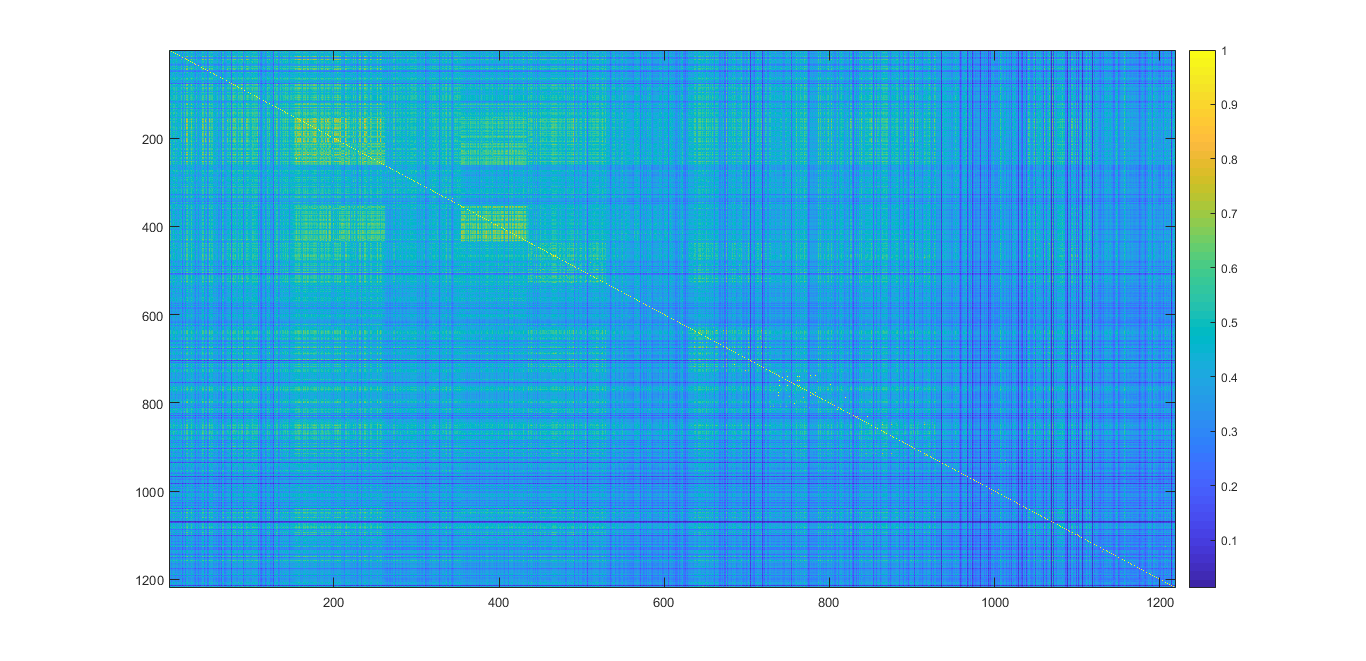
\includegraphics[width=1\linewidth]{figures/GaussianKernelIMG.png}
		\caption{Gaussian Kernel\label{FigGaussianKernel}}
	\end{subfigure}%
	\begin{subfigure}{.5\textwidth}
		\centering
		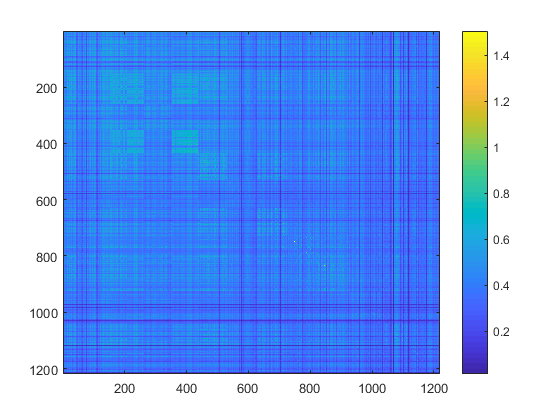
\includegraphics[width=1\linewidth]{figures/TKLKernelIMG.png}
		\caption{\acs{TKL} Kernel\label{FigTKLKernel}}
	\end{subfigure}
	\caption[Scatter Plot of Gaussian- and TKL-Kernel]{A scatter plot of the Gaussian and the \acs{TKL} kernel. On the left side the Gaussian kernel is shown. On the right, the \acs{TKL} kernel is shown. It is observable that the differences of source and target sets are slightly aligned. The kernel is based on the image set. This figure is best viewed with colors.\label{FigKernelComparison}}
\end{figure}
\section{PCTKVM Algorithm}\label{InSecAlgo}
In this section, the \acl{PCTKVM} algorithm will be discussed in detail.
As shown above, we have obtained our transfer learning kernel with the \acs{TKL} algorithm (\ref{PseudoCodeTKL}).
According to \cite{Long.2015} the new kernel can be feed to any kernel machine.
This means that we can train the regular \acf{PCVM} with our new kernel.
To train it we are using the extrapolated training kernel which is.
\begin{equation}
	\expP{\mathbf{K}}_\mathcal{Z} = \expP{\mathbf{U}}_\mathcal{Z}\mathbf{\Lambda}\expP{\mathbf{U}}_\mathcal{Z}^T
\end{equation}
However, simply using it in the \acs{PCVM} algorithm (\ref{PseudoCodePcvm}) has some disadvantages.
Revisiting the \acs{PCVM} algorithm, the kernel is recalculated in every iteration based on the optimized theta from the previous iteration.
As a consequence, we have to recalculate the entire transfer kernel too.
The complexity of the \acs{PCVM} is $\mathcal{O}(B^3)$ with $B$ as a number of basis functions.
We consider the worst case and substitute the number of basis function with the number of training samples $N$, which results in $\mathcal{O}(N^3)$.
The complexity of the \acs{TKL} is $\mathcal{O}((D+R)(N+M)^2)$, where $R$ is the number of eigenvectors and is $D$ is the dimension of the data. Combining these two, we would end up with a computational complexity of $\mathcal{O}(N^3(D+R)(N+M)^2)$.
This might be resulting in a long computational time.
In fact, the question is, whether we explicitly need the theta optimization in every iteration or not.
However, one advantage of the \acs{PCVM} was, to optimize the parameters within and therefore omit the need for a parameter optimization via grid search.
Furthermore, the performance of the \acs{PCTKVM} depends a lot from the quality of the theta, which can be seen in figure \ref{FigPerfomanceTheta}.
To keep this advantage and the performance up, a new approach must be found.
One approach could be to optimize the theta in not every iteration.
However, this seems to be no good solution, because we have observed that the theta is just dangling around the initial value, where we optimized the theta in every 5 or 10 iterations and nevertheless was leading in our tests to a worse performance, rather than just use a fixed value for theta.
The latter option would be to set the theta to a fixed value and omit the theta optimization completely.
Fair enough we can observe a good performance, which can be seen in section \ref{EmChap}.
Furthermore, we could obtain the complexity of $\mathcal{O}(N^3+(D+R)(N+M)^2)$.
If we consider $D$ as negligible because $D \ll N$, $R$ as constant and by multiplying out, we obtain $\mathcal{O}(N^3+M^2)$ for the \acs{PCTKVM} with a fixed theta.
For large $D$ we obtain $\mathcal{O}(N^3+DM^2)$.
\begin{figure}
	\centering
		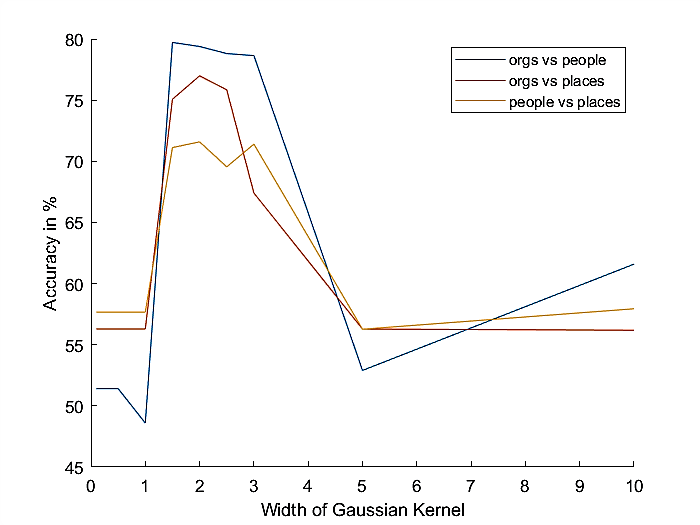
\includegraphics[width=.8\linewidth]{figures/PerformanceGaussianKernel.png}
	\caption[Perfomance in Dependence of Theta]{The performance of the \acs{PCTKVM} algorithm for different thetas shown as accuracy in \% which is evaluated on the Reuters dataset. It shows that the performance of the algorithm depends a lot on the quality of the theta.}
	\label{FigPerfomanceTheta}
\end{figure}
\FloatBarrier
\subsection{Theta Estimation}\label{InSubSecTheta}
\begin{figure}[t]
	\centering
	\begin{subfigure}{.5\textwidth}
		\centering
		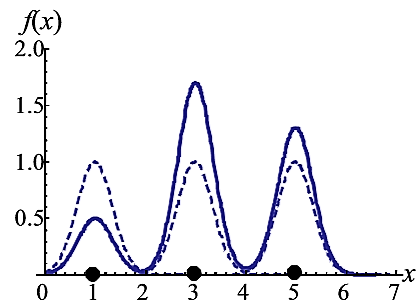
\includegraphics[width=1\linewidth]{figures/GaussianWidthSmall.png}
		\caption{Small Value \label{FigSmallWidth}}
	\end{subfigure}%
	\begin{subfigure}{.5\textwidth}
		\centering
		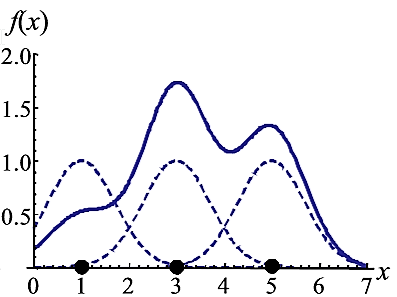
\includegraphics[width=1\linewidth]{figures/GaussianWidthLarge.png}
		\caption{Large Value \label{FigLargeWidth}}
	\end{subfigure}
	\caption[Effect of Width in Gaussian Kernel for Regression]{The effect of regression concerning the width of the Gaussian kernel. The left figure shows the effect of a width of 0.5. The right plot has used one as width. The black dots representing the data, the dashed lines are the Gaussian kernel, and the solid lines represent the regression. It can be seen that the larger width provides a smoother regression.\cite{Kitayama.2011}}
	\label{FigGaussianWidthRegression}
\end{figure}
Another, more deterministic but heuristic, approach to obtain a theta is presented by Kitayama in \cite{Kitayama.2011} and is discussed in the following.\\
It is important to notice that is just a simple estimation and therefore the optimal theta may not be found with this approach.\\
The width of the Gaussian kernel can play an important role not only for the \acs{PCVM} but many other algorithms.
Defining a 'good' value for the width leads to a more useful function which is observable in figure \ref{FigGaussianWidthRegression}.\cite{Kitayama.2011}
In this the black dots representing the data, the dashed lines are the Gaussian kernel, and the solid lines represent the regression.
In  \ref{FigSmallWidth} the width is set to 0.5 and in \ref{FigLargeWidth} it is set to 1.\newline
They are claiming in general that solving the theta via an optimization problem is very time-consuming.
The reason for this is because the optimization problem is depending on the data function, which can give a very large amount of variables and therefore proposed a simpler algorithm to find a good $\theta$.\cite{Kitayama.2011}\\
First, they use a scaling technique to scale every dimension to an equal range.
Consider $K = N + M$ as the number of all samples with $D$ dimensions.
In the approach, they using a \textit{Min-Max} normalization to do it:\cite{Kitayama.2011}
\begin{equation}
	x_j = \frac{x_j - x_j^L}{x_j^U-x_j^L} \times s, \>\>\> i=1,\dots,D 
\end{equation}
Where $x_j^L$ is the lower bound and $x_j^U$ is the upper bound of value and $s=\alpha\times s \alpha \ge 0$.
The $s$ is the abort criterion, but not needed in our approach.
The author's recommendation is to set alpha to 1.1.
Moreover, in every iteration of the algorithm, the dimension are rescaled.\\
However, in general, the training and test data for the \acs{PCVM} must be z-scored, as discussed in section \ref{Pc}.
Therefore, it seems reasonable to replace the scaling technique from \textit{Min-Max} to the z-score, obtained for example from \cite{Mohamad.2013}:
\begin{equation}\label{EqZTrans}
x_{ij} = Z(x_{ij}) = \frac{x_{ij}-\mean{x}_j}{\sigma_j},\>\>\> i=1,\dots,K \>\>\> j=1,\dots,D
\end{equation}
Where $\mean{x}_j$ is the mean and $\sigma_j$ is the standard deviation in every dimension.\\
Furthermore, because after one run of z-score the mean is 0 and the standard deviation is 1.\cite{Mohamad.2013}
Revisiting \eqref{EqZTrans} with this, we obtain $x_{ij} = Z(x_{ij}) = \frac{x_{ij}}{1}$ after the first run, which is the same for every following iteration.
With this change, we omitted the need for further iteration and can calculate the width in one iteration.\\
After the z-score is applied, and the dimensions are equally scaled they originally continue with determining the distance:\cite{Kitayama.2011}
\begin{equation}\label{EqMaxDist}
	\theta_i = \frac{d_{i,max}}{\sqrt{D}\sqrt[D]{K-1}}, i=1,\dots,K
\end{equation}
Where $d_{j,max}$ is the maximum distance between the $i$-th data point and another data point.
Moreover, $\theta_i$ is the width for the $i$-th Gaussian kernel in every row.\\
This is the main improvement in comparison with other approaches to determine the width because for example $\theta =\frac{d_{max}}{\sqrt[K]{KD}}$ can only be applied to uniform distributed data.
However, with \eqref{EqMaxDist} the distance can also be applied to non-uniform distributed data, which is mostly the case in real-world problems.\cite{Kitayama.2011}\newline
Finally, we set our width to the smallest maximal distance found in \eqref{EqMaxDist}.
The estimate can be summarized in the following steps based on \cite{Kitayama.2011}:
\begin{enumerate}[label=\bfseries Step \arabic*:,leftmargin=*,labelindent=1em]
	\item Rescale data using z-score from \eqref{EqZTrans}
	\item Calculate the distance matrix
	\item Find maximum distance for $K$ data points using \eqref{EqMaxDist}
	\item Find the minimum distance for every row with $\displaystyle\theta_{min}=\min_{1 \le i \le K}\theta_i$ and return $\theta_{min}$
\end{enumerate}
To calculate the distance in practice, we are using a dissimilarity matrix $\mathbf{D}_{K,K}$.
This matrix employs the Euclidean distance with $d_{i,j}=||x_i-x_j||^2, \forall i,j \in \mathbf{D}$ as dissimilarity measure.
This matrix is symmetric and is zero on the diagonal.\cite[p. 22;299]{Gentle.2007}\newline
Because the Gaussian kernel is used in this approach, the dissimilarity matrix is already involved in the computational complexity.
Therefore, this matrix has just to be calculated once and can be reused in the theta estimation and the Gaussian kernel.
Another important thing to notice is that the data is already z-scored in the preparation and therefore there is no need to do it twice.
With this, we just search the maximum distance with the built-in MatLab function \textit{min()} and can proceed with \eqref{EqMaxDist} in Step 3.\\
Although we can reduce the complexity with a clever implementation, the complexity discussion is based on the worst case involving all steps to compute, except z-score.
The computational complexity of calculating the dissimilarly matrix is $\mathcal{O}(K^2)$.\cite{Kobti.2007}
Furthermore, finding a maximum in $K$ rows with $D$ values can be solved in $\mathcal{O}(KD)$.
Because the dissimilarity matrix is symmetric the complexity changes to $\mathcal{O}(K^2)$ and multiplying a scalar to $K$ elements costs $\mathcal{O}(K)$, which can be summarized in $\mathcal{O}(K^2+K)=\mathcal{O}K^2)$.
Again finding a minimum within the theta array from step four takes $\mathcal{O}(K)$.
Summarizing, we can obtain the complexity of the theta estimation with $\mathcal{O}(K^2)$.
Note that we observed for small datasets, that the theta would be large, which will eventually lead to a worse performance, see section \ref{EmSecDaDes} and table \ref{TableThetaEst}.
\subsection{Training Algorithm}\label{InSubSecTraining}
With the results from the previous section, the \acs{PCTKVM} is presented in algorithm \ref{PseudoCodePCTKVM}.
\begin{algorithm}
	\caption{Probabilistic Classification Transfer Kernel Vector Machine (Short)}\label{PseudoCodePCTKVM}	
	\begin{algorithmic}[1]
		\Require Input Data $\mathbf{K} = [\mathbf{Z};\mathbf{X}]$ as $N$ sized training and $M$ sized text set; $\mathbf{Y}$ as $N$ sized training label vector; kernel(-type) \textit{ker}; eigenspectrum dumping factor $\zeta$; $\theta$ as kernel parameter; \textit{niter} as maximal number of iterations; \textit{threshold} $\tau$ as convergence criteria; \textbf{InitVector} as $N$-sized initialization vector.
		\Ensure Weight Vector $\mathbf{w}$; bias $b$, kernel parameter $\theta$; transfer kernel $\expP{\mathbf{K}}_\mathcal{A}$.
		\State $\mathbf{D}$ = calculate\_Dissimilarity\_Matrix($\mathbf{K}$);
		\State $\theta$ = theta\_Estimation($\mathbf{D}$);  \Comment{According to section \eqref{InSubSecTheta} (optional)}
		\State $\expP{\mathbf{K}}_\mathcal{A}$ = transfer\_Kernel\_Learning($\mathbf{D}$,\textit{ker},$\theta$,$\zeta$); \Comment{According to \eqref{InSecTrans}}
		\State [$\mathbf{w}$,$b$] = pcvm\_Training($\expP{\mathbf{K}}_\mathcal{Z}$,\textbf{InitVector},\textit{niter},$\tau$); \Comment{Algorithm \eqref{PseudoCodePcvm}}
	\end{algorithmic}
\end{algorithm}
Note that the complete algorithm which involves every detail can be found in appendix \ref{appac}. As already discussed, we are reusing the dissimilarity matrix. Therefore, the function parameters of \textit{transfer\_kernel\_Learning($\mathbf{D},\cdot$)} from the \acs{TKL} algorithm (\ref{PseudoCodeTKL}) changing from using the raw data to using the dissimilarity matrix.  
We observed in practice that the kernel is for some $\theta$, not \acs{PSD} anymore, although he is in theory.\cite{Long.2015}
We assume that there is some issue in the floating point multiplication for small numbers in MatLab and therefore added the regularization term $eps\mathbf{I}_{K\times K}$ to the kernel, which solved the problem.\\
It can be seen that the number of free parameters remains the same because the $\theta$ is estimated and only the eigenspectrum dumping factor $\zeta$ is left.
Furthermore, we obtain by, combining the complexity of the theta estimation with the complexities of \acs{PCVM} and \acs{TKL}, the same complexity as already discussed, which is $\mathcal{O}(N^3+M^2)$. Again, for a large $D$ we obtain $\mathcal{O}(N^3+DM^2)$.
This is achieved by reusing the dissimilarity matrix for the parameter estimation and the kernel function.
This statement can be validated in practice with table \ref{TableMeanTimeRank}, which shows that the \acs{PCTKVM} version with fixed theta and the algorithm with estimation need a similar time.
\subsection{Prediction}\label{InSubSecPrediction}
Additionally, we can make predictions based on the provided prediction function of the \acs{PCVM} with the use of $\expP{\mathbf{K}}_\mathcal{XZ} = \mathbf{U}_\mathcal{X}\mathbf{\Lambda}\expP{\mathbf{U}}_\mathcal{Z}^T$ as the kernel for prediction.\cite{Long.2015}\\
Because of the sparsity of the \acs{PCVM}, the kernel size is greatly reduced as discussed in section \ref{Pc}.
If we consider that our model has $B$ non-zero weight vectors with $B < N$ and because the \acs{PCVM} uses only kernel rows/columns corresponding to the non-zero weight vector index, then our final kernel $\expP{\mathbf{K}}_\mathcal{BX}$ for prediction has size $B\times M$.
Therefore, the prediction function of the \acs{PCTKVM} has the form:
\begin{equation}
\mathbf{y} = \expP{\mathbf{K}}_\mathcal{BX}\mathbf{w}+b
\end{equation}
Finally, the class label is obtained from the sign of the elements $y_i$ the label vector $\mathbf{y}_\mathcal{X}$, which has size $M$.\\
Note that the \acs{TKL} transforms the data into an \acs{RKHS}.
Bases on the reproducing property of an \acs{RKHS}, any additional target points could be integrated into the kernel.\cite{Long.2015}
Moreover, they can be evaluated with the \acs{PCTKVM}.\\
However, consider that new target points, which are evaluated after the calculation of the transfer kernel, should be drawn from the same marginal distribution as the previous target data. 
If this is prerequisite cannot be held, then the whole kernel has to be recalculated with the old and the composition of target data to obtain proper performance.\\
The probabilistic output is calculated with the probit link function as the \acs{PCVM} does it in equation \ref{EqPcGausLike}.

\subsection{Extensions}\label{InSubSecExt}
In the course of this work, there was the need to implement a multi-class option for the \acs{PCVM}, \acs{PCTKVM} and \acs{PCTKVM}\textsubscript{$\theta$Est}, because the Image dataset has more than two classes.\\
In general, there are many approaches to solve a multi-class problem for vector machines.\cite[p. 113]{Abe.2010}
According to the LibSVM documentation\footnote{\url{http://www.csie.ntu.edu.tw/~cjlin/libsvm/faq.html\#f419}}, for the LibSVM Library, two approaches are considered: The one vs. all and the one vs. one approach.
In the following, we will discuss the advantages and disadvantages for these two ideas and explain how it is integrated into the \acs{PCVM}.\\
The first is the one vs. rest approach.
Note that in the literature, the term one vs. all appears instead of one vs. rest.
If we consider $C$ classes, then the classifier would be trained with one class against the $C-1$ remaining classes.
This approach will have $C$ iteration, and in every iteration, another class is trained against every remaining class.
The label assignment for one class is done in one iteration only.
However, this will lead to large unclassifiable regions in the feature space.\cite[p. 114-116]{Abe.2010}\newline
Therefore, the second approach, one vs. one is implemented.
With this, we split up the labels in the different classes and train the classifier with every class against the others.
Again, if we take $C$, different classes, then our number of iteration is $I=C(C-1)/2$.
Furthermore, the unclassifiable region in comparison with the one vs. rest approach is smaller.
For the prediction, we do $I$ iterations again and predict the whole dataset with two classes.\cite[p. 127-128]{Abe.2010}\newline
In the implementation, consider a test set with size $M$.
Then our label matrix $\mathbf{Y}$ and the probabilistic output matrix $\mathbf{P}$ has size $M\times K$.\\
We choose a final label for the final label vector $\mathbf{y}$ by counting the number of occurrences of a label for a data point.
The data point is then assigned to the label which the classifier has assigned the most.
In case of a tie the smaller class label, in terms of numbers, is assigned, according to the MatLab \textit{mode}\footnote{\url{https://de.mathworks.com/help/matlab/ref/mode.html}} function.
This is rather unconventional because it is likely to be a random selection, but in our tests, the results are the better as to assign the class label according to the biggest probability given from $\mathbf{P}$.\\
To determine a final probability output for a final label decision concerning a data point, the algorithm calculates the mean of the probabilistic output for the runs, where the label is equal to the final label, which is assigned.\\
The number of relevance vectors is determined by counting all unique vectors, which are used during the $C$ iterations.

\section{Conclusion}\label{InSecCon}
In this chapter, we successfully integrated transfer learning in the \acs{PCVM}.
We used a proposed transfer learning method within the \acs{PCVM}, which forms the \acs{PCTKVM}.
Furthermore, we solved the problem that the algorithm will be slow through the theta optimization by adopting a simple theta estimation and adjust it to the needs of the \acs{PCVM}.
Because it uses unlabeled target data, the algorithm is transductive and solves the transfer problem with a relational-knowledge approach regarding homogeneous transfer learning.\\
Additionally, we extend the \acs{PCVM} and \acs{PCTKVM} to being able to solve multi-class problems via the one vs. one approach.
The MatLab source code of the \acs{PCTKVM} and \acs{PCTKVM}\textsubscript{$\theta$Est} can be obtained from Github\footnote{\url{https://github.com/ChristophRaab/pctkvm.git}}.
Furthermore, the reader can find the complete code written for this thesis, including all tests and transfer learning approaches used in the study, in the repository.
